% Adjust these for the path of the theme and its graphics, relative to this file
%\usepackage{beamerthemeFalmouthGamesAcademy}
\usepackage{../../beamerthemeFalmouthGamesAcademy}
\usepackage{multimedia}
\graphicspath{ {../../} }

% Default language for code listings
\lstset{language=C++,
        morekeywords={each,in,nullptr,int32, TCHAR, uint8, int8, uint16, int16,
        uint32, int32, uint64, int64, PTRINT, UObject. AActor, SWidget, FName,
        FString, UClass, USoundCue, UTexture}
}

% For strikethrough effect
\usepackage[normalem]{ulem}
\usepackage{wasysym}
\usepackage{listings}
\usepackage{pdfpages}

% http://www.texample.net/tikz/examples/state-machine/
\usetikzlibrary{arrows,automata}

\newcommand{\modulecode}{COMP260}\newcommand{\moduletitle}{Distributed Systems}\newcommand{\sessionnumber}{5}

\begin{document}
\title{\sessionnumber: 12}
\subtitle{\modulecode: \moduletitle}

\frame{\titlepage}

\begin{frame}
	\frametitle{Learning outcomes}
	\begin{itemize}
		\item \textbf{Identify} the various protocols used to communicate with devices attached to the Arduino
		\item \textbf{Explain} the difference between asynchronous \& synchronous communication
		\item \textbf{Outline} the strengths and weaknesses of each protocol
	\end{itemize}
\end{frame}

\begin{frame}
	\frametitle{Protocols}
	The main protocols used to communicate with devices from the Arduino
	\begin{itemize}
		\item \textbf{I2C} - The Inter-integrated Circuit (I2C) Protocol
		\item \textbf{SPI} - Serial Peripheral Interface
		\item \textbf{Dallas one-wire} - microLan
	\end{itemize}
\end{frame}

% ARDUINO I2C
\begin{frame}
	\frametitle{I2C Bus}
	\begin{figure}
		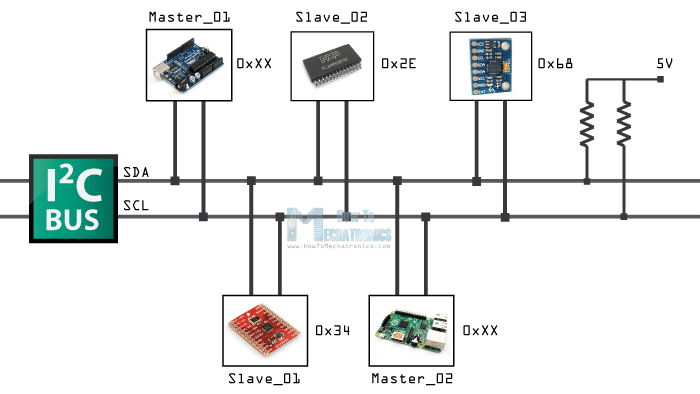
\includegraphics[scale=.35]{assets/i2c}  
	\end{figure}
	SCL is the clock line. It is used to synchronize all data transfers over the I2C bus. 
	SDA is the data line. 
	The SCL \& SDA lines are connected to all devices on the I2C bus
\end{frame}

\begin{frame}
	\frametitle{I2C Bus}
	\begin{figure}
		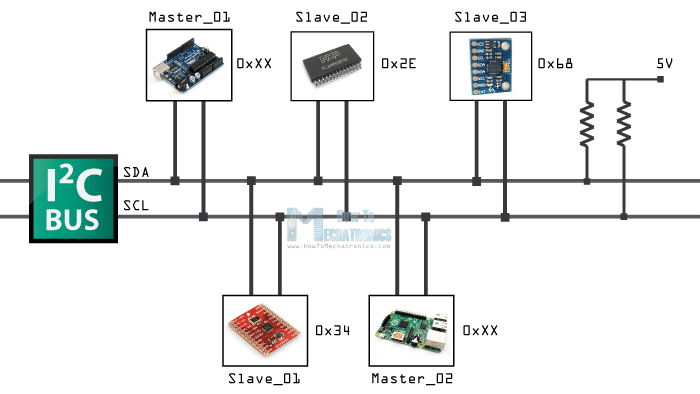
\includegraphics[scale=.25]{assets/i2c}  
	\end{figure}
	There should be a resistor from the SCL line to the 5v line and another from the SDA line to the 5v line. You only need one set of pull-up resistors for the whole I2C bus, not for each device. The value of the resistors is not critical. 1k8, 4k7 and 10k are common values.
\end{frame}

\begin{frame}
	\frametitle{I2C Bus}
	\begin{figure}
		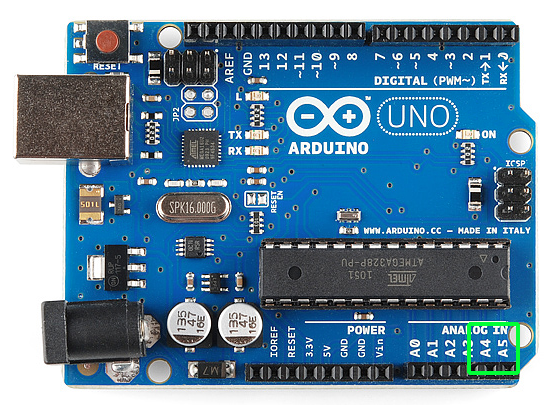
\includegraphics[scale=.35]{assets/i2carduino}  
	\end{figure}
	
	Uno uses pins A4 for SDA and A5 (SCL).
	I2C is easy to setup using the Wire Library preinstalled in the Arduino IDE.
\end{frame}


\begin{frame}
	\frametitle{Master \& Slaves}
The devices on the I2C bus are either masters or slaves. The master is always the device that drives the SCL clock line. The slaves are the devices that respond to the master. A slave cannot initiate a transfer over the I2C bus, only a master can do that. There can be, and usually are, multiple slaves on the I2C bus, however there is normally only one master.
\end{frame}

\begin{frame}
	\frametitle{I2C Experiment}
	\begin{figure}
		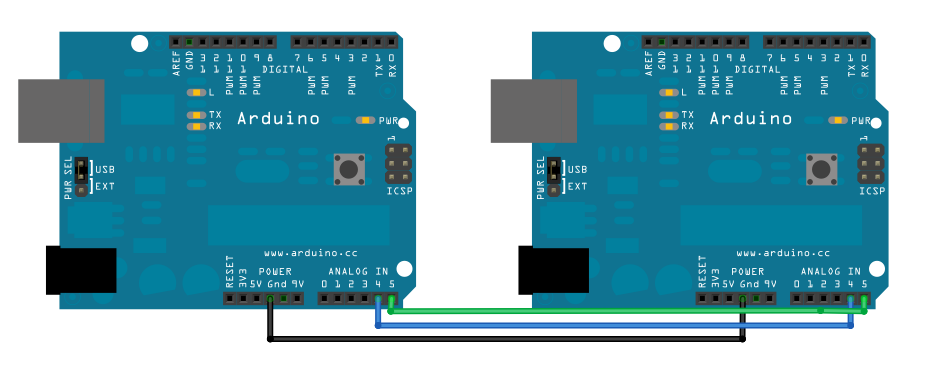
\includegraphics[scale=.2]{assets/arduino2arduino}  
	\end{figure}
	https://www.arduino.cc/en/Tutorial/MasterWriter
\end{frame}

% SPI

\begin{frame}
	\frametitle{SPI Bus}
	\begin{figure}
		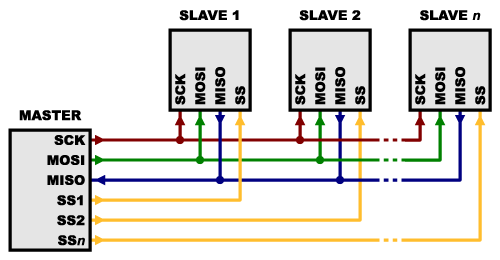
\includegraphics[scale=.15]{assets/spi}  
	\end{figure}
	\begin{itemize}
		\item \textbf{MISO} - (Master In Slave Out) - The Slave line for sending data to the master
		\item \textbf{MOSI} -  (Master Out Slave In) - The Master line for sending data to the peripherals,
		\item \textbf{SCK} - (Serial Clock) - The clock pulses which synchronize data transmission generated by the master
		\item \textbf{SS} - (Slave Select) - the pin on each device that the master can use to enable and disable specific devices.
	\end{itemize}
\end{frame}

\begin{frame}
	\frametitle{SPI Bus}
	\begin{figure}
		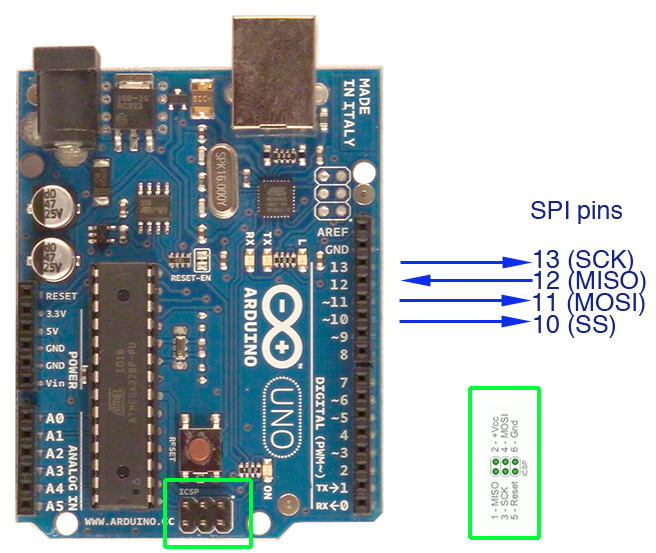
\includegraphics[scale=.25]{assets/spiarduino}  
	\end{figure}
	SPI is easy to setup using the SPI Library preinstalled in the Arduino IDE.
\end{frame}


\begin{frame}
	\frametitle{Master \& Slaves}
In general, each slave will need a separate SS line. To talk to a particular slave, you?ll make that slave?s SS line low and keep the rest of them high (you don?t want two slaves activated at the same time, or they may both try to talk on the same MISO line resulting in garbled data). Lots of slaves will require lots of SS lines; if you?re running low on outputs, there are binary decoder chips that can multiply your SS outputs.
\end{frame}


% Asynchronous VS. Synchronous 

\begin{frame}
	\frametitle{Asynchronous - SPI}
	\textbf{Asynchronous} means that data is transferred without support from an external clock signal. This transmission method is perfect for minimizing the required wires and I/O pins, but it does mean we need to put some extra effort into reliably transferring and receiving data.
\end{frame}


\begin{frame}
	\frametitle{Synchronous - SPI}
	A \textbf{synchronous} serial interface always pairs its data line(s) with a clock signal, so all devices on a synchronous serial bus share a common clock. This makes for a more straightforward, often faster serial transfer, but it also requires at least one extra wire between communicating devices. Examples of synchronous interfaces include SPI, and I2C.

\end{frame}

%MAXIM one wire - Neo Pixels
\begin{frame}
	\frametitle{Dallas One-wire \& NeoPixels}
	Other protocols to watch for!
	\begin{figure}
		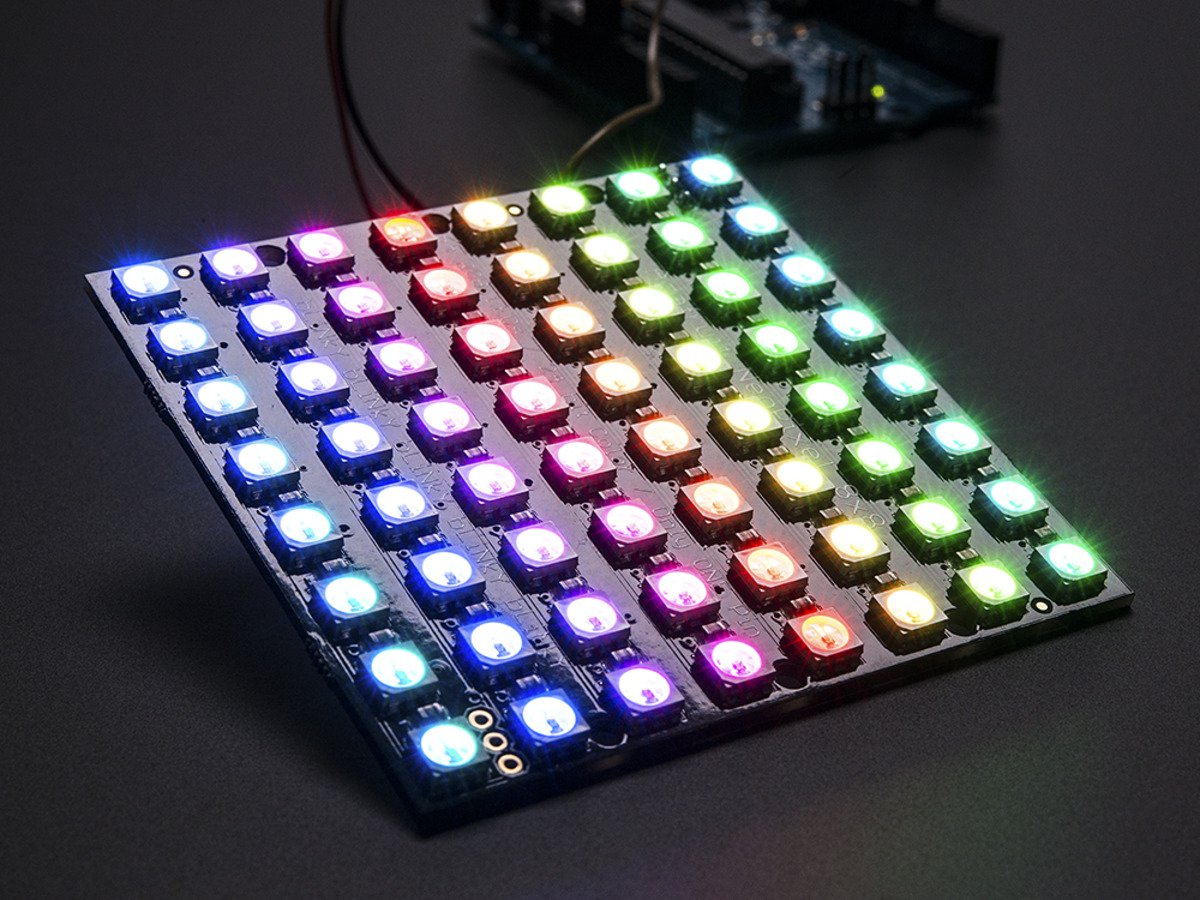
\includegraphics[scale=.4]{assets/neo}  
	\end{figure}

\end{frame}


\begin{frame}
	\frametitle{Emulate USB Keyboard}
	\begin{figure}
		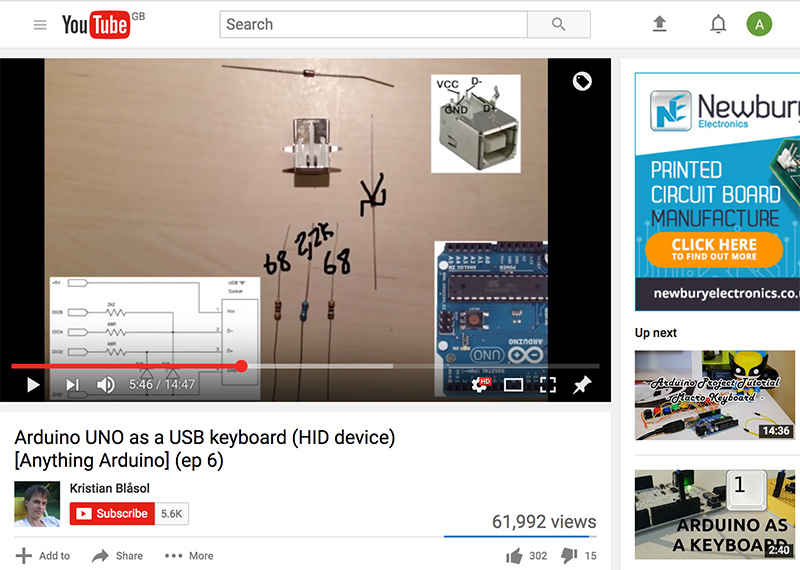
\includegraphics[scale=.4]{assets/keyboard}  
	\end{figure}
	\url{https://www.youtube.com/watch?v=RoG_-9lAnSI}
\end{frame}


%https://www.youtube.com/watch?v=RoG_-9lAnSI uno keyboard emulation

\end{document}
